






\begin{minipage}{0.49\textwidth}
  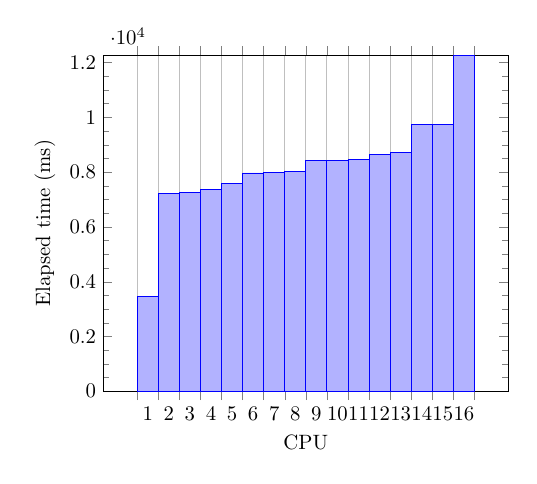
\begin{tikzpicture}[scale=0.75]
    \begin{axis}[ybar interval, ymax=12274,ymin=0, minor y tick num = 3, xlabel={CPU}, ylabel={Elapsed time (ms)}]
      \addplot coordinates {(1,3459) (2,7231) (3,7252) (4,7353) (5,7584) (6,7970) (7,7996) (8,8034) (9,8432) (10,8441) (11,8462) (12,8643) (13,8714) (14,9739) (15,9755) (16,12274) (17,0)};
     \end{axis}
  \end{tikzpicture}
  \caption*{Repeats  + kassian load balancing}
\end{minipage}
\begin{minipage}{0.49\textwidth}
  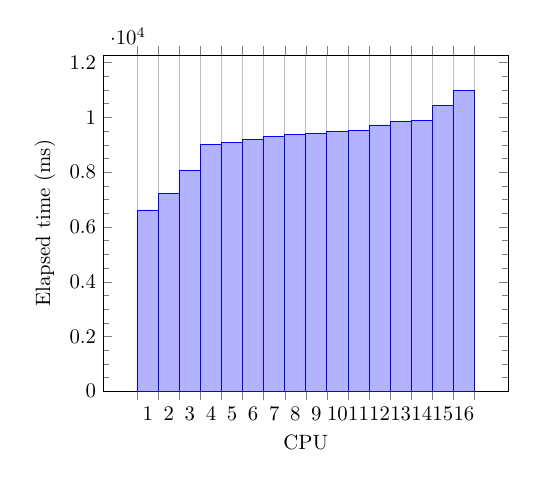
\begin{tikzpicture}[scale=0.75]
    \begin{axis}[ybar interval, ymax=12274,ymin=0, minor y tick num = 3, xlabel={CPU}, ylabel={Elapsed time (ms)}]
      \addplot coordinates {(1,6621) (2,7210) (3,8053) (4,9006) (5,9079) (6,9196) (7,9312) (8,9386) (9,9424) (10,9493) (11,9509) (12,9723) (13,9858) (14,9878) (15,10449) (16,10992) (17,0)};
     \end{axis}
  \end{tikzpicture}
  \caption*{Repeats  + randomized load balancing}
\end{minipage}


\begin{minipage}{0.49\textwidth}
  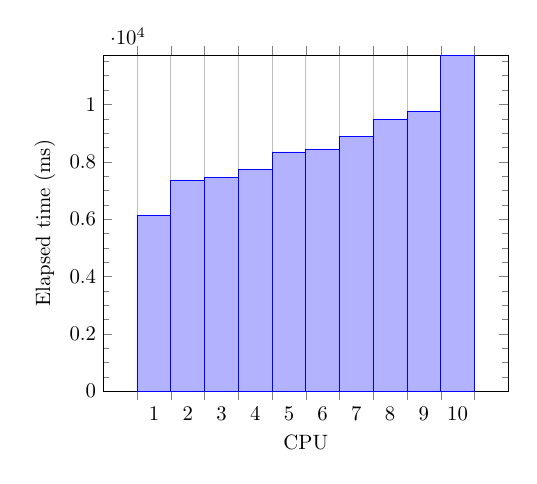
\begin{tikzpicture}[scale=0.75]
    \begin{axis}[ybar interval, ymax=11718,ymin=0, minor y tick num = 3, xlabel={CPU}, ylabel={Elapsed time (ms)}]
      \addplot coordinates {(1,6114) (2,7361) (3,7438) (4,7730) (5,8341) (6,8440) (7,8867) (8,9462) (9,9745) (10,11718) (11,0)};
     \end{axis}
  \end{tikzpicture}
  \caption*{Repeats  + kassian load balancing}
\end{minipage}
\begin{minipage}{0.49\textwidth}
  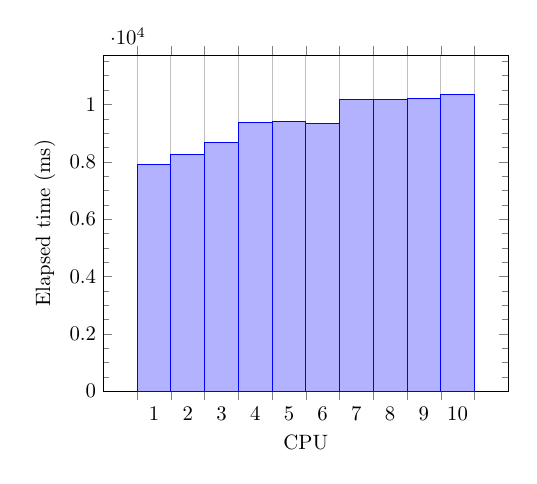
\begin{tikzpicture}[scale=0.75]
    \begin{axis}[ybar interval, ymax=11718,ymin=0, minor y tick num = 3, xlabel={CPU}, ylabel={Elapsed time (ms)}]
      \addplot coordinates {(1,7903) (2,8265) (3,8677) (4,9367) (5,9414) (6,9344) (7,10162) (8,10181) (9,10204) (10,10341) (11,0)};
     \end{axis}
  \end{tikzpicture}
  \caption*{Repeats  + randomized load balancing}
\end{minipage}
